Throughout the development of Yarn, acceptance tests and specifications were
written prior to developing a feature. This provided a solid test coverage
which in turn allowed for some radical refactorings to improve the quality,
readability and performance of the system. By the end of development, all
12 acceptance tests and 77 specifications passed. The final test coverage was
94.38\%, as depicted on Figure~\ref{coverage}. 

\begin{figure}[htb]
  \centering
  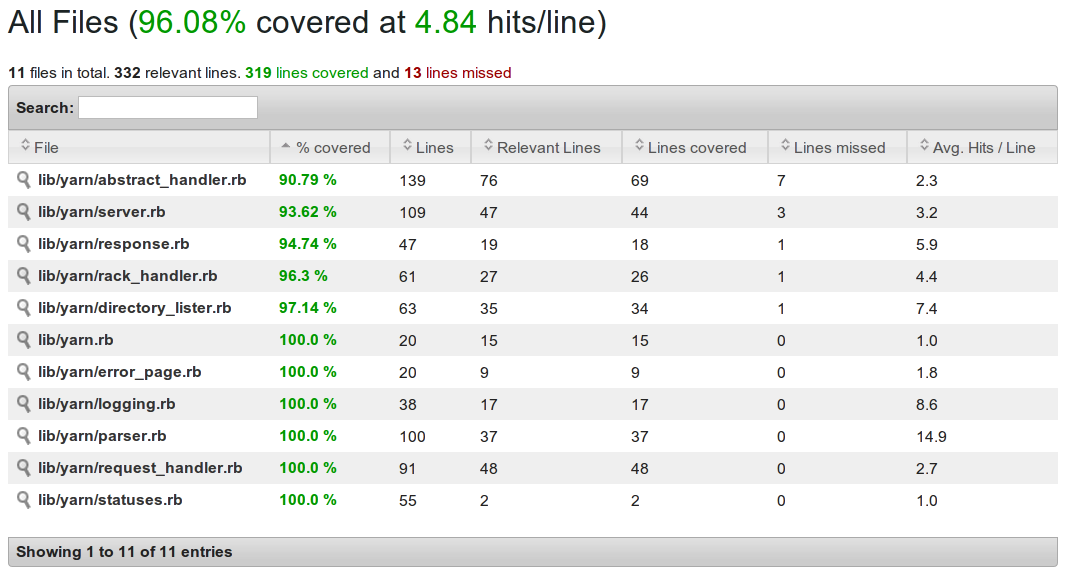
\includegraphics[width=1.0\textwidth]{img/coverage.png}
  \caption{Yarn test coverage screenshot.}
  \label{coverage}
\end{figure}

During the development, the test coverage was continously monitored to ensure
all parts of the system was exercised in the test suite. The test coverage
analysis is available on the CD in the \texttt{coverage} folder. 

